% Write about what kind of queries you are expect to get in this system
\section{The execution of the database queries}
List of situation the database administrator is to expect and what are the types of execution for the database when this occur
% Write more information about this section
\begin{itemize}
\item User creates post
\item User comments post
\item User creates message
\item User receives message
\item User adds friend (relation)
\item User receives friend request
\item 
\end{itemize}

\subsection{User creates a new post}
The database is expected to create a new data which is added into the tables including any necessary relations that relates to the post.

\subsection{User comments post}

\section{Database table layout}
NB: Public keys are 217 characters long, all id's are auto-incremented.

\begin{table}[h]
    \centering
    \begin{tabular}{ll}
    attribute      & description\\ \hline
    id \textbf{PK} & \\
    username       & \\
    name           & \\
    birthday       & \\
    sex            & \\
    e-mail         & \\
    public\_key    & \\
    \end{tabular}
    \caption{table: users}
\end{table}

\begin{table}[h]
    \centering
    \begin{tabular}{ll}
    attribute            & description\\ \hline
    id \textbf{PK}       & \\
    user\_id \textbf{FK} & \\
    name                 & \\
    \end{tabular}
    \caption{table: category}
\end{table}

\begin{table}[h]
    \centering
    \begin{tabular}{ll}
    attribute                           & description\\ \hline
    id \textbf{PK}                      & \\
    permission\_allowed\_to \textbf{FK} & this list of users are permissible to view the post, its comments and likes\\
    from \textbf{FK}                    & \\
    to \textbf{FK}                      & this can be NULL if the wall is not posted for a specific person\\
    comment\_id                         & \\
    content                             & \\
    time                                & \\
    \end{tabular}
    \caption{table: wall\_post}
\end{table}

\begin{table}[h]
    \centering
    \begin{tabular}{ll}
    attribute      & description\\ \hline
    id \textbf{PK} & \\
    login\_time    & \\
    logout\_time   & \\
    \end{tabular}
    \caption{table: login\_logout\_log}
\end{table}

\begin{table}[h]
    \centering
    \begin{tabular}{ll}
    attribute               & description\\ \hline
    message\_id \textbf{PK} & \\
    from \textbf{FK}        & \\
    to \textbf{FK}          & \\
    content                 & \\
    time                    & \\
    \end{tabular}
    \caption{table: private\_message}
\end{table}

\begin{table}[h]
    \centering
    \begin{tabular}{ll}
    attribute            & description\\ \hline
    id \textbf{PK}       & \\
    post\_id \textbf{FK} & from wall\_post table\\
    comment\_from        & \\
    comment\_time        & \\
    \end{tabular}
    \caption{table: comment}
\end{table}

\begin{table}[h]
    \centering
    \begin{tabular}{ll}
    attribute              & description\\ \hline
    id \textbf{PK}         & \\
    post\_id \textbf{FK}   & \\
    like\_from \textbf{FK} & \\
    \end{tabular}
    \caption{table: like}
\end{table}

\begin{table}[h]
    \centering
    \begin{tabular}{ll}
    attribute                           & description\\ \hline
    id \textbf{PK}                      & \\
    title                               & \\
    content                             & \\ 
    from \textbf{FK}                    & \\
    permission\_allowed\_to \textbf{FK} & \\
    \end{tabular}
    \caption{table: events}
\end{table}

\begin{figure}[h]
    \centering
    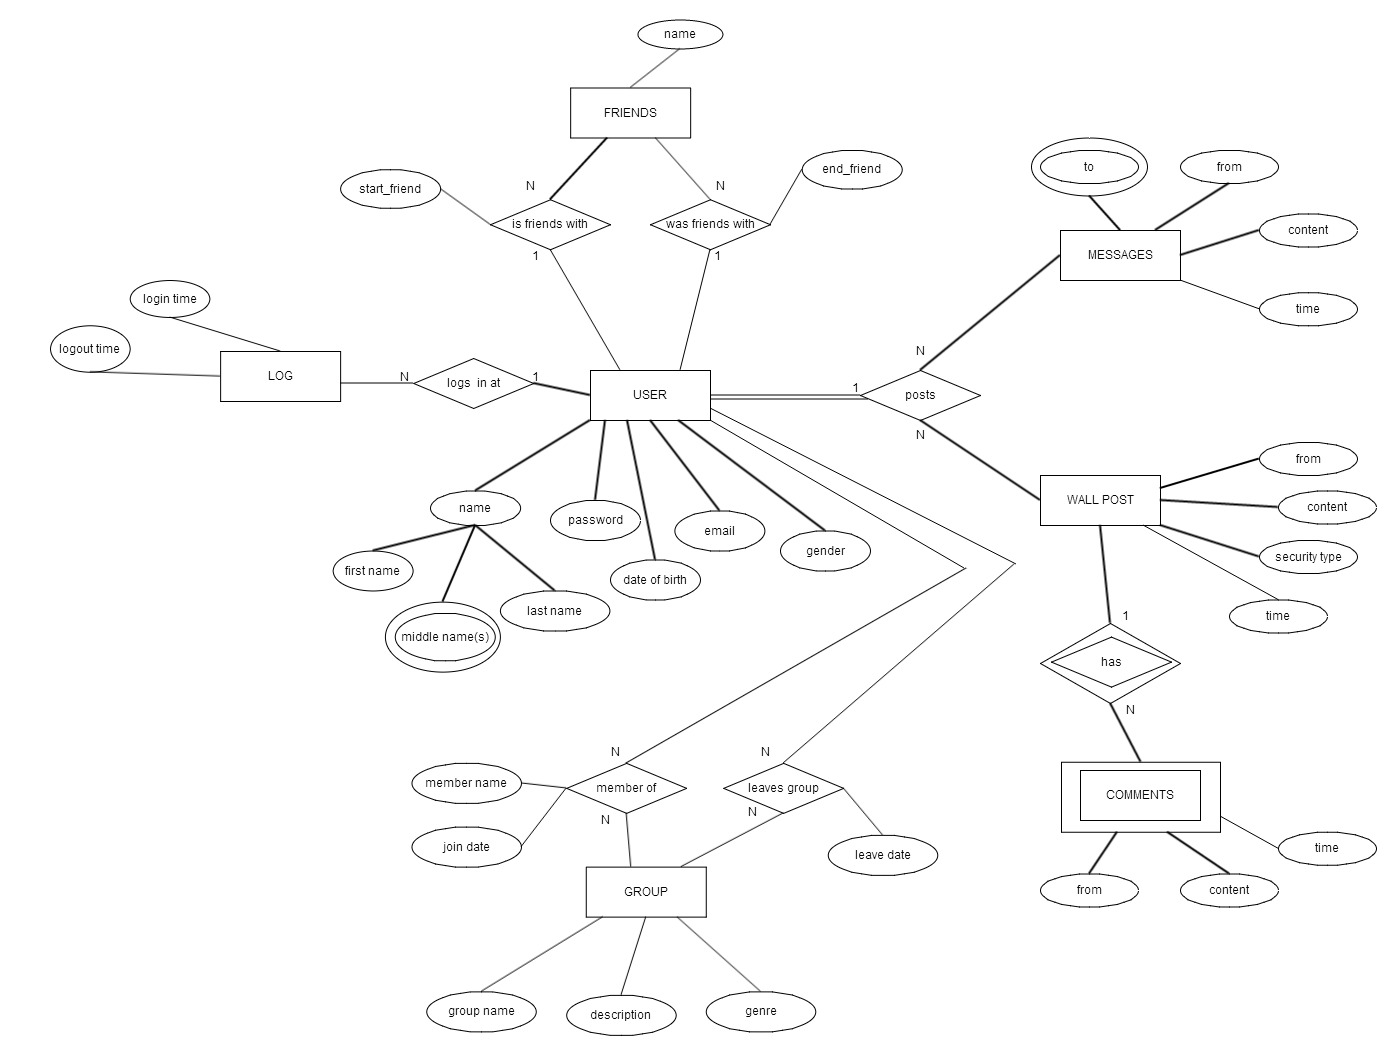
\includegraphics[width=\textwidth]{images/design/er_diagram.jpg}
    \caption{Database E-R Diagram}
    \label{fig:db_er_diag}
\end{figure}
